\section{Analysis and Interpretability}

\subsection{Embedding Space Topology via t-SNE}
Figure~\ref{fig:tsne_comparison} presents two-dimensional t-SNE projections~\cite{tsne} of feature embeddings for the four species of the \textit{Afzelia} genus (\textit{A.~africana}, \textit{A.~bella}, \textit{A.~pachyloba}, and \textit{A.~quanzensis}). 

\begin{figure}[H]
\centering
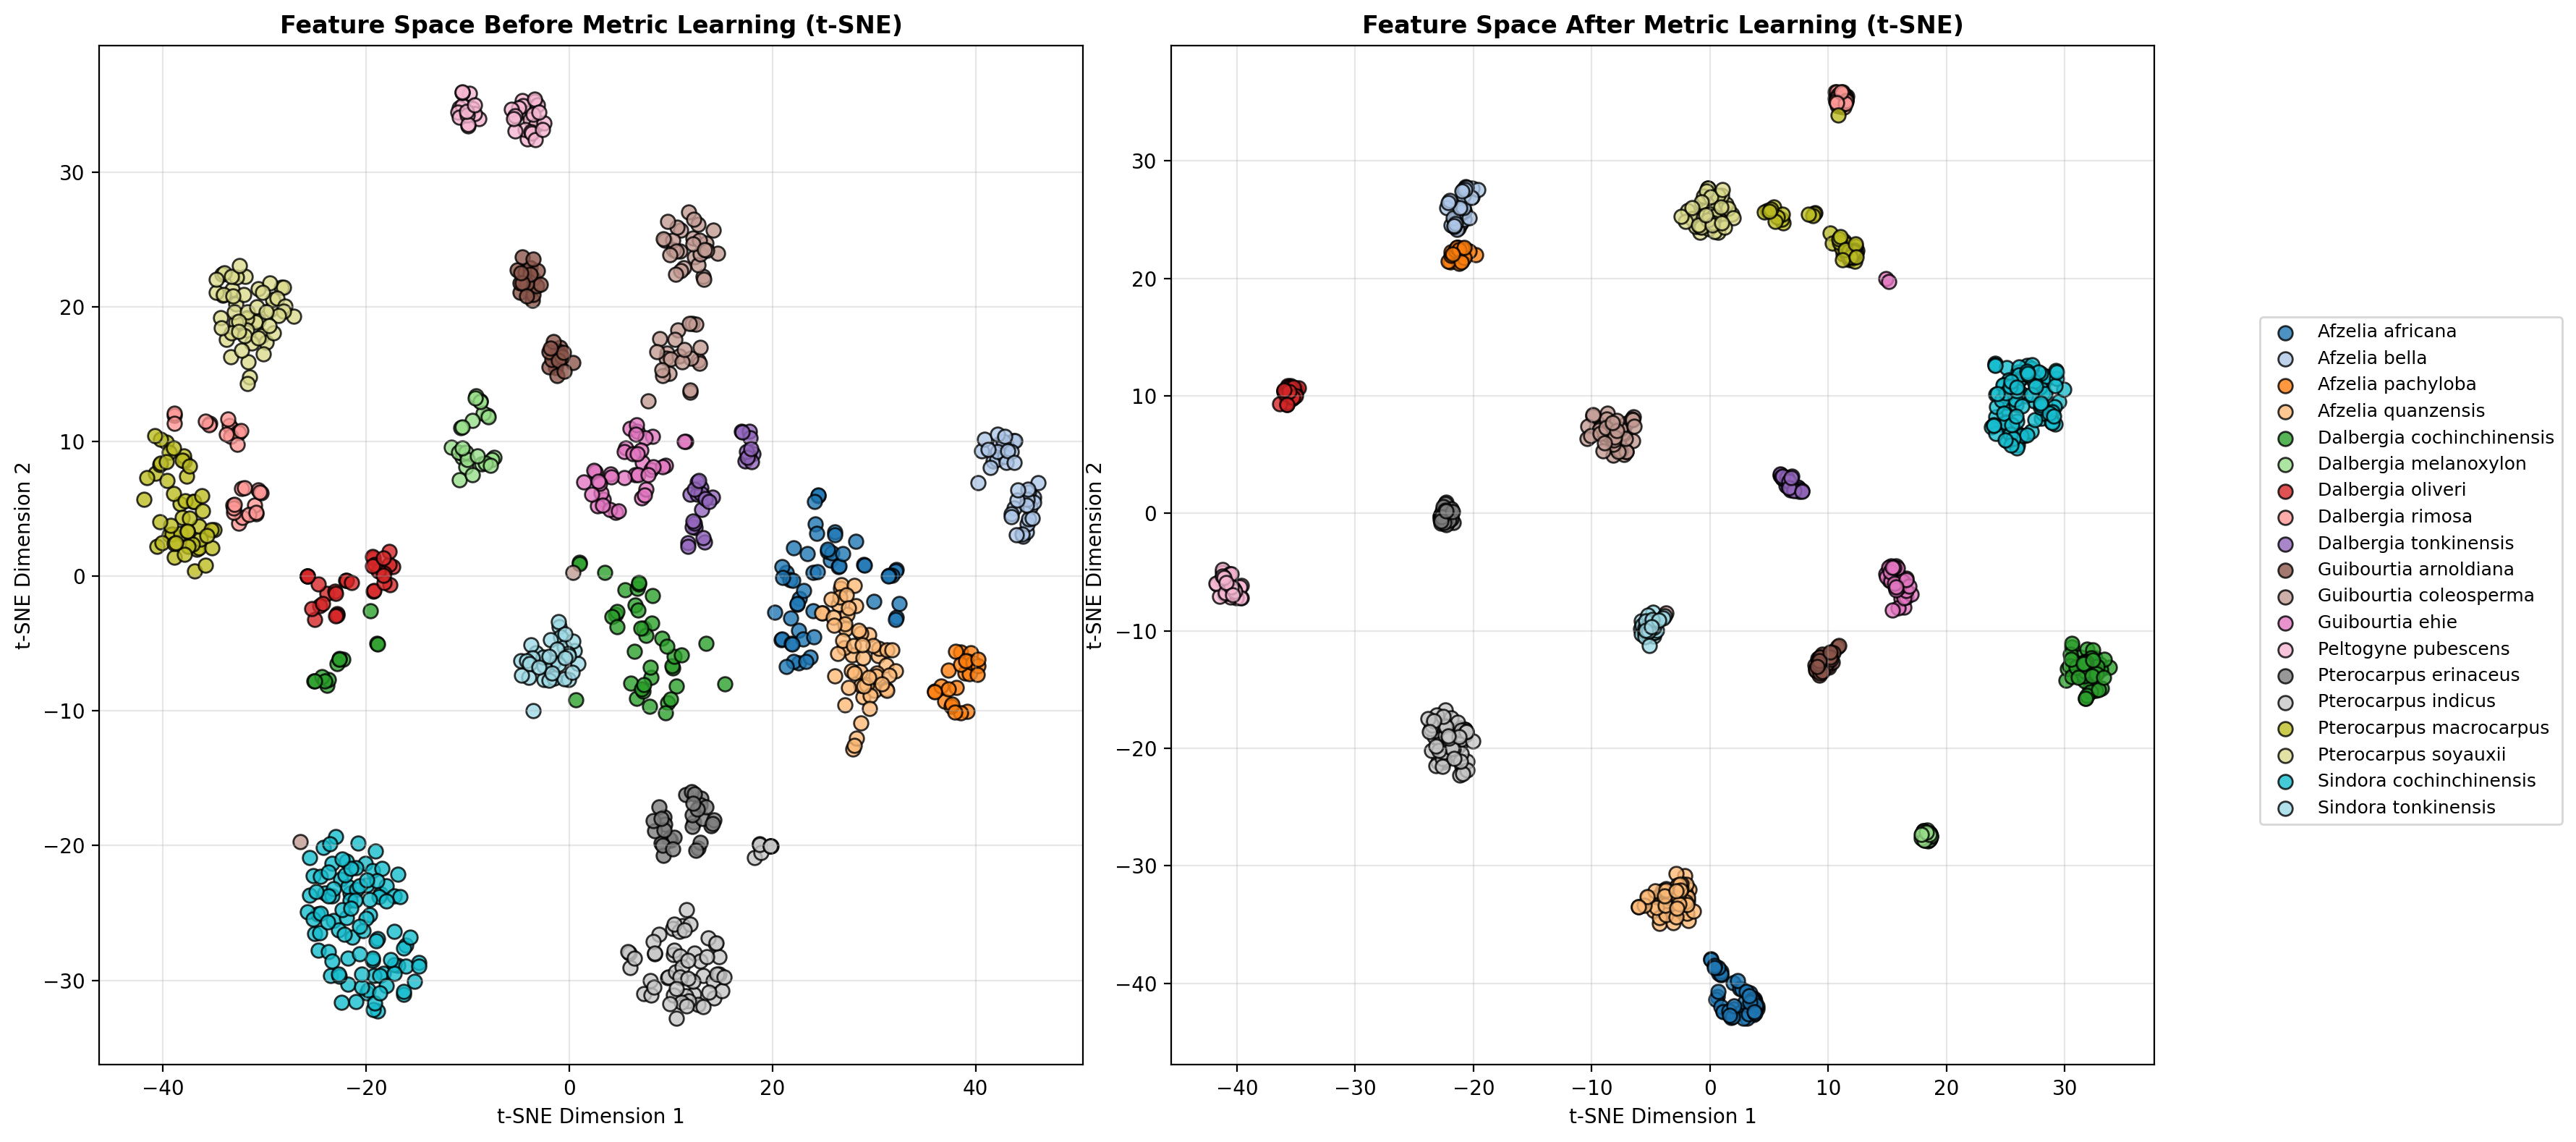
\includegraphics[width=0.75\textwidth]{fig/tsne_comparison.png}
\caption{t-SNE embedding projections for the \textit{Afzelia} genus comparing feature distribution under Random Image Split (left, exhibiting artificial clustering due to specimen leakage) against held-out physical specimens under CEGS-Split (right).}
\label{fig:tsne_comparison}
\end{figure}

Under random image-level partitioning (left), feature embeddings for sibling species appear cleanly separated because the network memorizes specimen-specific background shortcuts. However, when evaluating on held-out physical specimens under CEGS-Split (right), the embeddings for \textit{A.~bella} and \textit{A.~pachyloba} display substantial spatial overlap, explaining their low F1-scores (\textbf{0.0260} and \textbf{0.2708}) and revealing true biological intra-genus similarity.

\subsection{Pairwise Distance Distribution Analysis}
Figure~\ref{fig:distance_distribution} illustrates the empirical probability density functions of intra-class (same-species) and inter-class (different-species) Euclidean distances in feature space. For $L_2$-normalized embeddings $\mathbf{z}_i, \mathbf{z}_j \in \mathbb{S}^{D-1}$, Euclidean distance relates directly to cosine similarity via:
\begin{equation}
d_{ij} = \|\mathbf{z}_i - \mathbf{z}_j\|_2 = \sqrt{2(1 - \mathbf{z}_i^T \mathbf{z}_j)}.
\end{equation}

\begin{figure}[H]
\centering
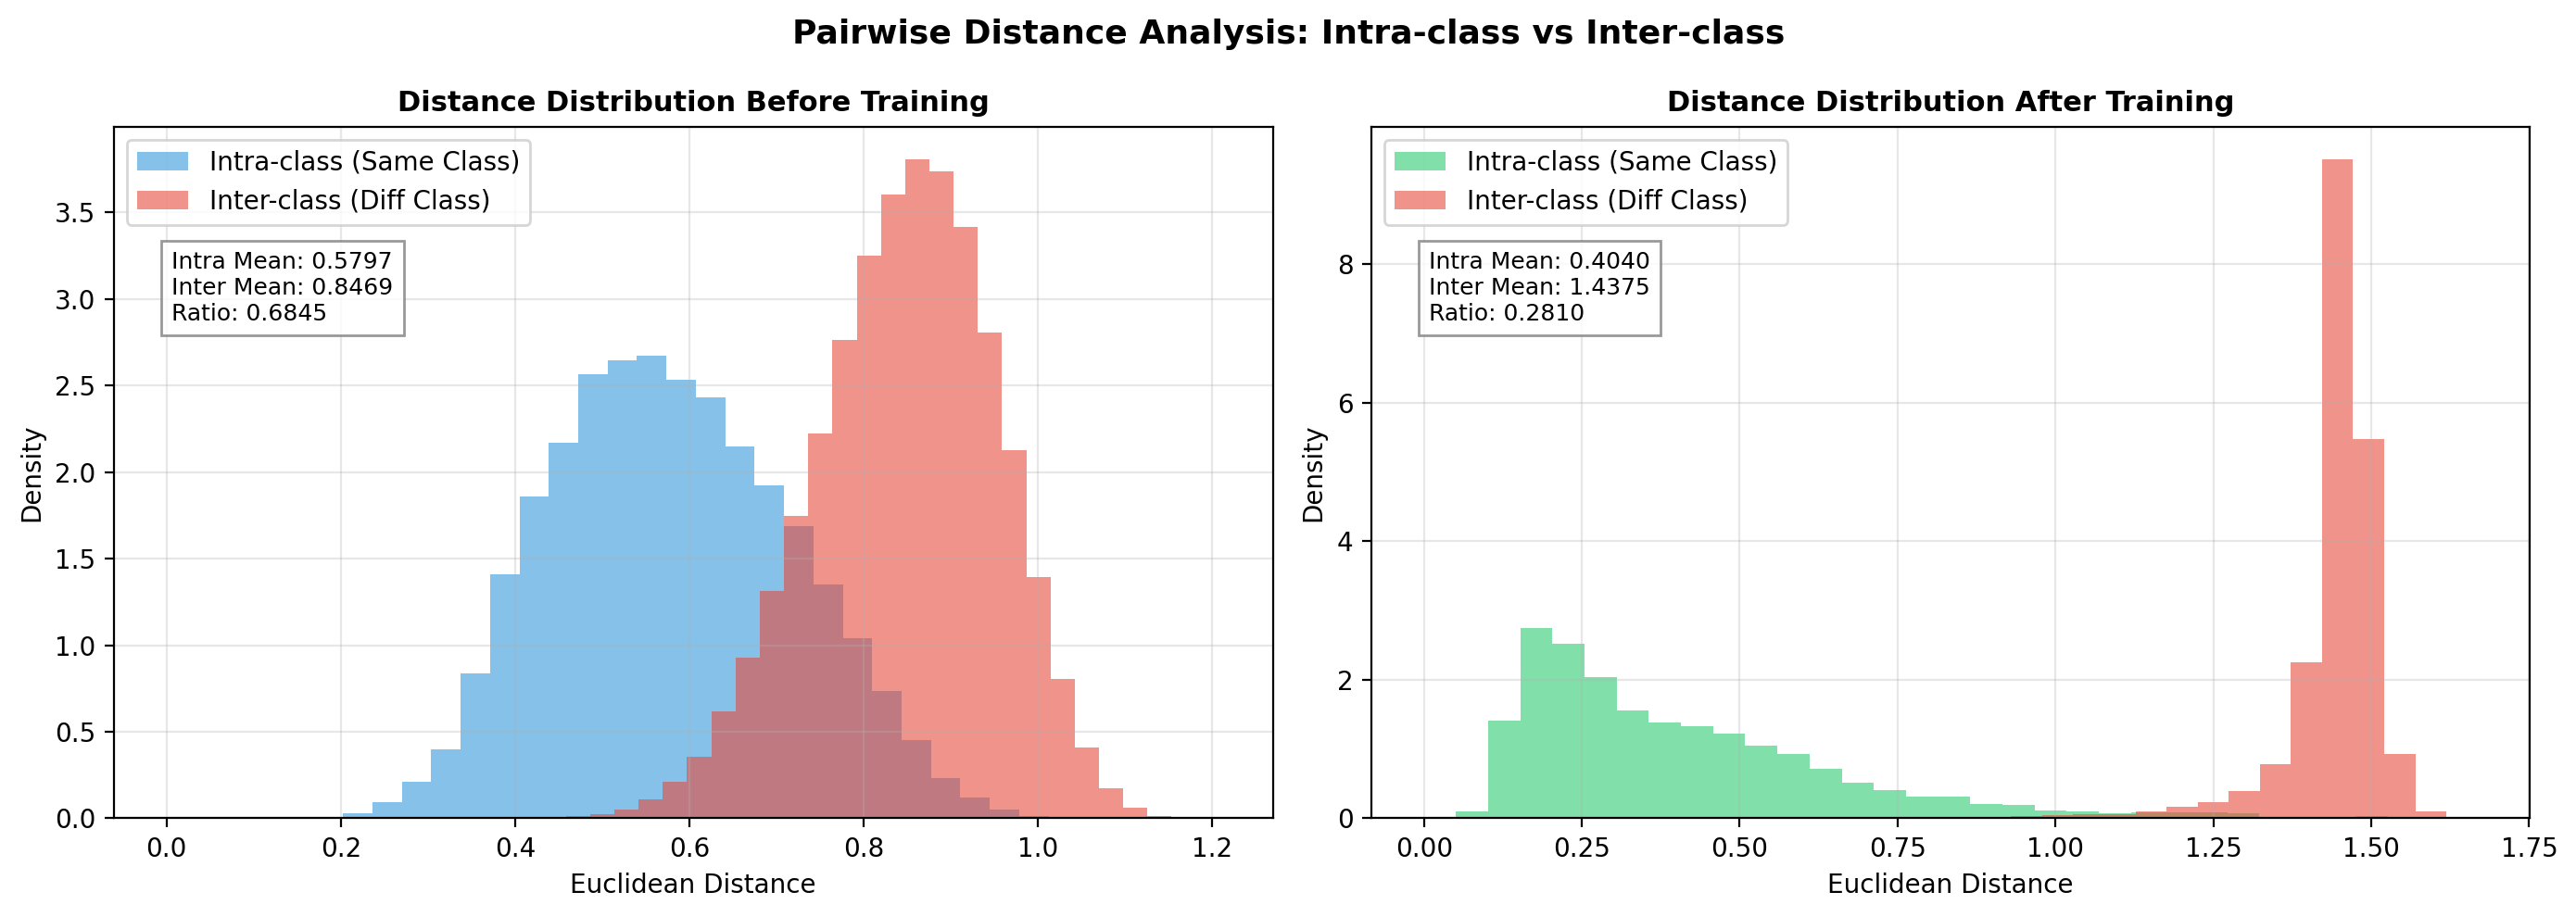
\includegraphics[width=0.75\textwidth]{fig/distance_distribution.png}
\caption{Probability density functions of intra-class vs. inter-class Euclidean distances under Random Split (leakage) versus CEGS-Split (specimen-disjoint).}
\label{fig:distance_distribution}
\end{figure}

Under random image splits, near-duplicate images originating from identical physical specimens create an artificially sharp intra-class distance peak near $d_{ij} \to 0$, giving a false impression of compact, easily separable feature clusters. Under CEGS-Split, the true biological intra-class variance is revealed, demonstrating that evaluation protocols must enforce specimen isolation to prevent artificial cluster sharpening.

\subsection{Attention Map Auditing and Shortcut Learning}
To investigate whether models learn genuine biological features or non-taxonomic shortcuts under different partitioning protocols, we visualize Grad-CAM~\cite{gradcam} feature attribution maps (Figure~\ref{fig:grad_cam}).

\begin{figure}[H]
\centering
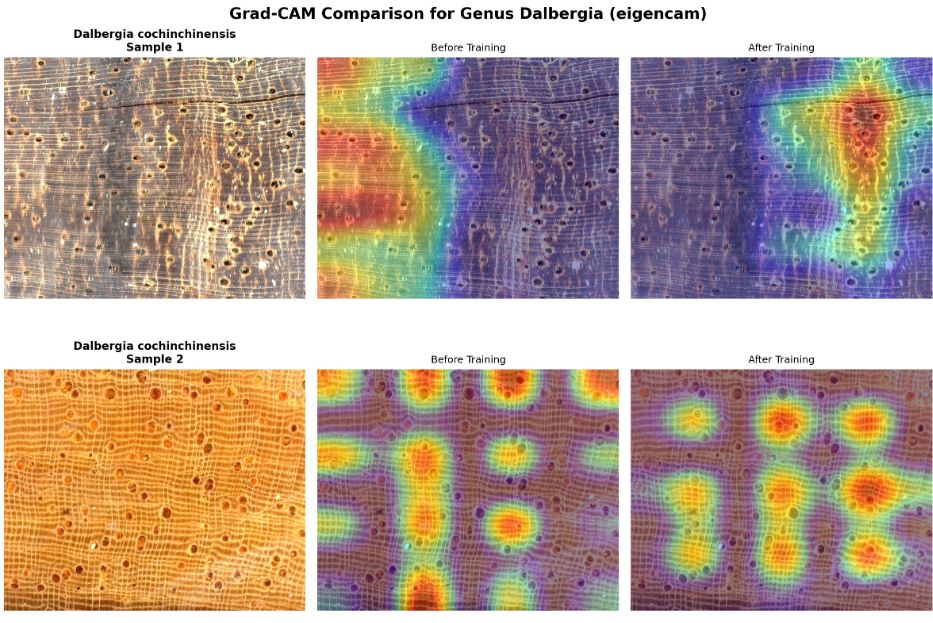
\includegraphics[width=0.85\textwidth]{fig/grad-cam.png}
\caption{Qualitative comparison of Grad-CAM attention maps: model trained under Random Image Split (top, exhibiting shortcut memorization on saw marks and edges) vs. model trained under Specimen-Disjoint CEGS-Split (bottom, focusing on vessel pores and axial parenchyma).}
\label{fig:grad_cam}
\end{figure}

Diagnostic visual inspection highlights two contrasting behaviors:
\begin{itemize}
\item \textbf{Random Split Shortcut Memorization}: Networks trained under random image splits frequently focus on \emph{non-taxonomic artifacts}---such as mechanical saw scratches, sanding grit patterns, specimen edge borders, optical illumination gradients, and camera sensor noise. The network acts as a "Clever Hans" predictor re-identifying known wood blocks.
\item \textbf{Specimen-Disjoint Feature Grounding}: When trained under specimen-disjoint governance (CEGS-Split), networks are forced to ignore block-specific shortcuts and instead focus activation strictly on \emph{diagnostic anatomical structures recognized by xylotomists}: solitary and grouped vessel pores, axial parenchyma bands, and wood ray orientations.
\end{itemize}

This visual evidence confirms that specimen-level data governance encourages neural networks to learn anatomically grounded representations that generalize to novel physical timber samples.
